\documentclass[12pt, a4paper, twoside, openright]{report}

%%─── Encoding & fonts ────────────────────────────────────────────────────────
\usepackage[T1]{fontenc}
\usepackage[utf8]{inputenc}
\usepackage{lmodern}  % sans-serif font (Helvetica)
\usepackage{microtype}

%%─── Page layout ─────────────────────────────────────────────────────────────
\usepackage[
  a4paper,
  top=2.5cm, bottom=2.5cm,
  left=2.5cm, right=2.5cm,
]{geometry}
\usepackage{setspace}
\onehalfspacing
\usepackage[section]{placeins}

%%─── Mathematics ─────────────────────────────────────────────────────────────
\usepackage{amsmath}
\usepackage{amssymb}
\usepackage{amsthm}
\usepackage{mathtools}
\usepackage{bm}
\usepackage{enumerate}  % [(i)] style list labels

%%─── Theorem-like environments ───────────────────────────────────────────────
\theoremstyle{plain}
\newtheorem{theorem}{Theorem}[chapter]
\newtheorem{proposition}[theorem]{Proposition}
\newtheorem{lemma}[theorem]{Lemma}
\newtheorem{corollary}[theorem]{Corollary}

\theoremstyle{definition}
\newtheorem{definition}[theorem]{Definition}
\newtheorem{example}[theorem]{Example}
\newtheorem{assumption}[theorem]{Assumption}

\theoremstyle{remark}
\newtheorem{remark}[theorem]{Remark}
\newtheorem{notation}[theorem]{Notation}

%%─── Graphics & tables ───────────────────────────────────────────────────────
\usepackage{graphicx}
\usepackage{booktabs}
\usepackage{array}
\usepackage{longtable}
\usepackage{subcaption}
\usepackage{xcolor}

%%─── Algorithms (requires texlive-science; install before use) ───────────────
% \usepackage[ruled, vlined, linesnumbered]{algorithm2e}

%%─── Bibliography ─────────────────────────────────────────────────────────────
\usepackage[round, authoryear, sort]{natbib}
\bibliographystyle{plainnat}

%%─── Hyperlinks (load before cleveref, after most packages) ──────────────────
\usepackage[hidelinks]{hyperref}
\usepackage[capitalize, noabbrev]{cleveref}

%%─── Headers & footers ───────────────────────────────────────────────────────
\usepackage{fancyhdr}
\pagestyle{fancy}
\fancyhf{}
\fancyhead[LE,RO]{\thepage}
\fancyhead[LO]{\nouppercase{\leftmark}}
\fancyhead[RE]{\nouppercase{\rightmark}}
\renewcommand{\headrulewidth}{0.4pt}
\fancypagestyle{plain}{%
  \fancyhf{}%
  \fancyfoot[C]{\thepage}%
  \renewcommand{\headrulewidth}{0pt}%
}

%%─── Epigraph (manual implementation; epigraph.sty not in basic install) ────
\newcommand{\epigraph}[2]{%
  \vspace{1em}%
  \begin{flushright}%
    \begin{minipage}{0.65\textwidth}%
      \itshape #1\\[4pt]%
      \upshape\small\hfill #2%
    \end{minipage}%
  \end{flushright}%
  \vspace{1.5em}%
}

%%─── Custom mathematical macros ──────────────────────────────────────────────
%% Number sets
\newcommand{\R}{\mathbb{R}}
\newcommand{\N}{\mathbb{N}}
\newcommand{\Z}{\mathbb{Z}}
\newcommand{\TT}{\mathbb{T}}          % time-index set

%% Probability / expectation
\renewcommand{\P}{\mathbb{P}}
\newcommand{\Prob}{\mathbb{P}}         % probability measure (overrides paragraph symbol)
\newcommand{\E}{\mathbb{E}}           % expectation
\newcommand{\Var}{\operatorname{Var}}
\newcommand{\Cov}{\operatorname{Cov}}

%% Sigma-algebras and filtrations
\newcommand{\F}{\mathcal{F}}          % generic sigma-algebra
\newcommand{\bbF}{\mathbb{F}}         % filtration as a family (\mathbb{F} = (\F_t))

%% Bold vectors / matrices
\newcommand{\bY}{\mathbf{Y}}
\newcommand{\bfR}{\mathbf{R}}         % bold R (missingness indicator); \R reserved for reals
\newcommand{\br}{\mathbf{r}}          % lower-case bold r (realization of \bfR)
\newcommand{\bX}{\mathbf{X}}
\newcommand{\bS}{\mathbf{S}}          % price vector
\newcommand{\bA}{\mathbf{A}}
\newcommand{\bB}{\mathbf{B}}
\newcommand{\bC}{\mathbf{C}}
\newcommand{\bD}{\mathbf{D}}
\newcommand{\bQ}{\mathbf{Q}}
\newcommand{\bI}{\mathbf{I}}          % identity matrix
\newcommand{\bzero}{\mathbf{0}}
\newcommand{\bone}{\mathbf{1}}

%% Bold Greek
\newcommand{\bmu}{\boldsymbol{\mu}}
\newcommand{\bSigma}{\boldsymbol{\Sigma}}
\newcommand{\bPhi}{\boldsymbol{\Phi}}
\newcommand{\bTheta}{\boldsymbol{\Theta}}
\newcommand{\bepsilon}{\boldsymbol{\varepsilon}}
\newcommand{\bnu}{\boldsymbol{\nu}}
\newcommand{\btheta}{\boldsymbol{\theta}}
\newcommand{\bpsi}{\boldsymbol{\psi}}

%% Indicator (bold 1 subscript; no bbm package required)
\newcommand{\indic}[1]{\mathbf{1}_{\!\left\{#1\right\}}}

%% Misc operators
\DeclareMathOperator{\tr}{tr}
\DeclareMathOperator{\diag}{diag}
\DeclareMathOperator{\rank}{rank}

%%─── Document begins ──────────────────────────────────────────────────────────
\begin{document}


%%━━━━━━━━━━━━━━━━━━━━━━━━━━━━━━━━━━━━━━━━━━━━━━━━━━━━━━━━━━━━━━━━━━━━━━━━━━━
%% FRONT MATTER — Acknowledgements
%%━━━━━━━━━━━━━━━━━━━━━━━━━━━━━━━━━━━━━━━━━━━━━━━━━━━━━━━━━━━━━━━━━━━━━━━━━━━
\thispagestyle{empty}
\null
\clearpage

\thispagestyle{empty}
\null
\clearpage

%% --- Acknowledgements page -------------------------------------------------
\thispagestyle{empty}
\vspace*{\fill}
\begin{center}
	{\Large\itshape Acknowledgements}
\end{center}
\vspace{2em}
\begin{center}
\begin{minipage}{0.8\textwidth}
\itshape
....
\end{minipage}
\end{center}
\vspace*{\fill}
\clearpage

%% --- Intentionally blank page ----------------------------------------------
\thispagestyle{empty}
\null
\clearpage


%% --- Contents / figures / tables -------------------------------------------

\tableofcontents
\thispagestyle{empty}
\clearpage

\thispagestyle{empty}
\null
\clearpage




%%━━━━━━━━━━━━━━━━━━━━━━━━━━━━━━━━━━━━━━━━━━━━━━━━━━━━━━━━━━━━━━━━━━━━━━━━━━━
%% MAIN MATTER
%%━━━━━━━━━━━━━━━━━━━━━━━━━━━━━━━━━━━━━━━━━━━━━━━━━━━━━━━━━━━━━━━━━━━━━━━━━━━
\pagenumbering{arabic}

%%═══════════════════════════════════════════════════════════════════════════════
% =====================================================================
%  introduction.tex
%  Introduction chapter for a thesis on imputation of missing data in
%  sparse financial panels, evaluated by downstream model quality.
%
%  USAGE: This is a chapter FRAGMENT. Do NOT add \documentclass or a
%  preamble here. Include it from your report-class main.tex, e.g.
%
%      \documentclass[12pt]{report}
%      \usepackage{amsmath,amssymb}     % needed for the math below
%      % ... your bibliography setup (natbib / biblatex / plain bibtex)
%      \begin{document}
%      \include{introduction}           % or \input{introduction.tex}
%      ...
%      \end{document}
%
%  Citations use the package-agnostic \cite{} so this compiles under
%  natbib, biblatex, or plain BibTeX. The keys used here are listed at
%  the end of this file; matching .bib entries are provided separately.
% =====================================================================

\chapter{Introduction}
\label{chap:introduction}

\section{Motivation}
\label{sec:motivation}

Financial time series data is never fully observed.
Limit-order book feeds drop quotes during bursts of order cancellations.
Equity markets suspend trading when prices move too violently.
Over-the-counter bond markets leave entire yield-curve tenors unquoted
for days.
Implied volatility surfaces contain large regions where no liquid
option trade has occurred.
Macro and alternative data arrive at mixed, irregular frequencies, with
publication lags that create structural gaps at the daily level.
This missing data is pervasive and often elusive, and gets in the way
of advanced analysis. Thus practitioners or a researchers face
the same decision: what value should be attributed to the missing
observation, and how much uncertainty should be attached to that
attribution?

The simplest and most common solution is to carry forward the last observed value,
but this can lead to systematic mispricing, underestimation of risk, and distortion
of correlations among assets.

We aim to take a different path, one that looks for solutions that aim to preserve as much
as possible the statistical properties of the series, in order to maintain the integrity of
the underlying data and consequently the robustness of any downstream model that relies on it.
Since this can be considered an inference problem, we will also explore ML algorithms,
and in classical machine learning approach, we will
focus on quality of inference rather than interpretability of the model.

In this thesis we will test these different methods of imputation, and evaluate them not only on the
accuracy of the imputation itself (MSE,...),
but also on the quality of the downstream model that uses the imputed data, and how
far it deviates from the case where all data is observed.

\section{Literature review}
\label{sec:literature}

The modern theory of missing data originates with
\cite{rubin1976}, who classifies the mechanism that generates the gaps.
Let the complete data be partitioned into observed and missing parts,
$X = (X_{\text{obs}}, X_{\text{mis}})$, and let $R$ denote the matrix of
missingness indicators, governed by a conditional law $P(R \mid X,
\phi)$. The mechanism is \emph{missing completely at random} (MCAR) if
$R$ is independent of the data, \emph{missing at random} (MAR) if it
depends only on the observed part $X_{\text{obs}}$, and \emph{missing not
at random} (MNAR) if it depends on the unobserved values
$X_{\text{mis}}$ themselves. The practical importance of this taxonomy
lies in the \emph{ignorability} result: likelihood-based and Bayesian
inference may ignore the missingness mechanism if and only if the data
are MAR and the data and mechanism parameters are distinct
\cite{rubin1976,littlerubin2019}. This is the condition that licenses
the expectation--maximisation algorithm \cite{dempster1977} and multiple
imputation \cite{rubin1987} without explicitly modelling $R$.

Financial data violates the convenient end of this taxonomy. Missingness
in returns and fundamentals is typically MNAR and strongly structured:
it clusters in the cross section and persists over time, and the very
fact that a value is missing is informative about that value. Returns
themselves depend on whether data are missing
\cite{bryzgalova2025}. Two consequences follow directly and motivate the
methods studied here. First, complete-case analysis conditions on
survival and on disclosure, producing a sample that is not
representative of the population of interest. Second, unconditional mean
imputation, even where it leaves first moments unbiased, attenuates
estimated variances and covariances toward zero. Because mean--variance
portfolio selection and risk measurement consume the covariance matrix
$\Sigma$---and, through the optimiser, its inverse $\Sigma^{-1}$---this
attenuation corrupts exactly the object the downstream model depends
upon.

\section{From imputation to estimation: the downstream view}
\label{sec:downstream}

The clearest illustration of the downstream view, and the running
example of this thesis, is mean--variance portfolio selection
\cite{markowitz1952}, in which the optimal risky portfolio is
proportional to $\Sigma^{-1}\mu$ for a mean vector $\mu$ and covariance
$\Sigma$. It is well established that plugging sample estimates into this
expression performs poorly out of sample: the optimiser behaves as an
``error maximiser'', loading on assets whose moments are most favourably
mis-estimated \cite{michaud1989,jobsonkorkie1981}. The estimation-error
problem is severe enough that a naive equally weighted portfolio is hard
to beat \cite{demiguel2009}, and a large literature responds with
regularisation: shrinkage of the covariance matrix
\cite{ledoitwolf2004,ledoitwolf2017} or equivalent weight constraints
\cite{jagannathanma2003}.

Imputation enters this picture not as a separate preprocessing step but
as a further source of regularisation. Filling a return panel with a
low-rank or factor-based reconstruction shrinks the estimated covariance
toward a factor structure---the same target used deliberately by
shrinkage estimators. The choice of imputation method and the choice of
covariance estimator are therefore not separable, and the error that
imputation introduces propagates through $\Sigma^{-1}$ into the portfolio
weights and ultimately into realised performance. This is why
reconstruction accuracy is an inadequate criterion: it ignores how the
imputation interacts with the conditioning of the downstream estimator.
The natural evaluation is instead a two-layer one, comparing methods both
on reconstruction error and on a downstream objective such as realised
portfolio variance, Sharpe ratio, or tail risk, with particular interest
in the configurations where the rankings reverse.

Mean--variance optimisation is only the leading example. The same
impute-then-estimate logic governs risk-model estimation and the
computation of Value-at-Risk and Expected Shortfall; the estimation of
factor models and cross-sectional return predictors from panels of firm
characteristics \cite{freyberger2020,chenzimmermann2022}; volatility
forecasting; macroeconomic nowcasting from mixed-frequency, ragged-edge
data; the construction of yield curves and implied-volatility surfaces
from sparsely observed grids; and credit-risk and ESG scoring, where the
underlying data are both heavily and informatively missing. In each case
the relevant question is identical: how does the imputation choice change
the estimate that the practitioner actually uses.

\section{Sparse and illiquid markets}
\label{sec:emerging}

The problem sharpens in emerging and illiquid markets, where it also
changes in character. The dominant difficulty there is often not an
explicit missing cell but \emph{staleness}: an asset that does not trade
still carries a recorded closing price---yesterday's---so the panel can
appear fully observed while being silently contaminated by repeated
prices and spurious zero returns. The missingness is in part
\emph{latent}, inferred rather than flagged, which must be detected
before it can be addressed, for instance through the proportion of
zero-return days and related liquidity proxies
\cite{lesmond1999,amihud2002}. Whether a stale observation should be
treated as observed or converted to missing is itself a modelling
decision with downstream consequences.

Illiquidity also intensifies the statistical biases of interest.
Non-trading is more likely in adverse states of the world, so the
missing observations are disproportionately the extreme ones, which
inflates estimated means and understates downside risk. Non-synchronous
prices bias correlations and betas downward and understate volatility, so
that a portfolio optimiser fed stale data systematically understates risk
and overstates diversification; standard corrections estimate exposures
using leads and lags \cite{scholeswilliams1977,dimson1979}. Because the
characteristic failure mode is the under-statement of risk, evaluation in
this setting should emphasise realised downside measures rather than
in-sample Sharpe ratios alone. Finally, illiquidity yields a testable
prediction that the thesis examines: since the time series of an illiquid
asset is largely uninformative, cross-sectional and low-rank methods,
which borrow strength from contemporaneous liquid peers, should outperform
time-series fillers by a wider margin in emerging markets than in
developed ones.

\section{Research questions}
\label{sec:questions}


\section{Contributions}
\label{sec:contributions}


\section{Outline of the thesis}
\label{sec:outline}

\chapter{Methodology}
\label{ch:methodology}

As already mentioned, missing data can arise in countless different ways,
and the choice of methodology depends on the nature of the missingness, the type of data,
and the specific goals of the analysis. We will focus on a subset
of cases, namely those that involve imputation of the missing values with
"information" from the whole dataset (no causal constraint), with in mind
the goal of training a downstream model that is as close as possible to
the one that would have been trained on the complete dataset.
Our choice of data, models, and evaluation methods will be guided
by these constraints. We will nevertheless mention when/how models should
be tweaked to solve adjacent problems.

\section{Data}
\label{sec:data}

As our main baseline, we chose the most studied and reliable dataset in finance:
the end-of-day prices of the S\&P500, in this case fetched with yfinance from
1/1/2010 to 30/5/2026 (potrei cambiare le date). It clearly is not a dataset inflicted
with the curse of missing data; the only structural ones being occasional circuit breaks
and listings/delistings from the index. To obtain a full dataset with no "real"
missing data, we removed each stock that contained at least one missing observation.
Furthermore, we selected a sample of 50 stocks from the index, stratified across industries;
this is a sensible choice because:
\begin{enumerate}
    \item with more 400 stocks the covariance matrix $\Sigma$ quickly becomes unreliable (noisy covariances,
    skewed eigenvalues, unstable inversion\dots) as the number of observations shrinks;
    \item it is easier to check whether the ground data is actually correct;
    \item model training requires considerably less memory, in a time where RAM and GPU prices are 
    skyrocketing;
    \item it is well known that a well constructed portfolio with more than 30 stocks is already
    sufficiently diversified (since volatility scales with the inverse of the square root of the number of securities).
\end{enumerate}

This dataset will serve as the ground truth against which we will compare our results.
In parallel, we will modify it by inserting fake missing observations according to different
rules, as we define in the subsequent sections.
Now an important choice is whether to operate in the prices "space" or the returns space.
There are positives and negatives about each. For one, the raw dataset is prices, and
in practice missing data will come in the form of missing prices.
\section{Models}
\label{sec:models}

\section{Evaluation Methods}
\label{sec:eval}

%\section{Geometrical Interpretation}
\label{geometry}

In this section we want to develop some geometrical intuition behind the
evaluation methods criteria and the imputation models, as well as why a
missing data problem requires different methods from an usual inference
problem.

Take a multivariate time series of daily log returns:
\[
R =
\begin{pmatrix}
r_1^\top \\
r_2^\top \\
\vdots \\
r_T^\top
\end{pmatrix}
=
\begin{pmatrix}
r_{11} & r_{12} & \cdots & r_{1N}\\
r_{21} & r_{22} & \cdots & r_{2N}\\
\vdots & \vdots & \ddots & \vdots\\
r_{T1} & r_{T2} & \cdots & r_{TN}
\end{pmatrix}
\in\mathbb{R}^{T\times N}
\]

The (t)-th observation is:

\[
r_t =
(r_{t1},\ldots,r_{tN})^\top
\in\mathbb{R}^N
\]

The (i)-th variable asset realization is:

\[
R_i =
(r_{1i},\ldots,x_{Ti})^\top
\in\mathbb{R}^T
\]

Let us first consider each asset separately.
We interpret each asset return series as a finite-sample realization of an underlying square-integrable random variable
in a Hilbert space:

\[
R_i \in
L^2(\Omega,\mathcal{F},\mathbb{P})
=
\left\{
X:\Omega\rightarrow\mathbb{R}
:
\mathbb{E}[X^2]<\infty
\right\}
\]

Square integrability, which is a reasonable assumption \footnote{Empirical work as \cite{plerou1999} shows
that the power law exponent of individual stocks is around 3, meaning variance exists but skew and kurtosis may not.},
enables us to define an useful inner product
on $L^2$, namely:
\[
\langle X,Y\rangle
\eqqcolon
\mathbb{E}[XY]
\]

This is remarkably similar to the definition of covariance, and is equal when the mean
of $X$ and $Y$ is zero; at the daily level this is almost the case. We can use this
approximation to see that the covariance and correlation of two assets are a function
of their angle in $L^2$:

\[
\langle X,Y\rangle
\simeq
\operatorname{Cov}(X,Y)
\]

\[
\rho(X,Y)
=
\frac{\operatorname{Cov}(X,Y)}{\operatorname{Var}(X)\operatorname{Var}(Y)}
\simeq
\frac{\langle X,Y\rangle}
{\|X\|\|Y\|}
=\cos(\theta)
\]

The crucial part of this thesis is making sure that this linear geometry is preserved
when imputing the missing data. The covariance matrix is of course the main
object of discussion, especially since it is used so widely across finance. It is
immediate that MSE is the squared distance of two assets.
The other metrics like VaR have no easy interpretation in this space.

\begin{figure}

  \centering
  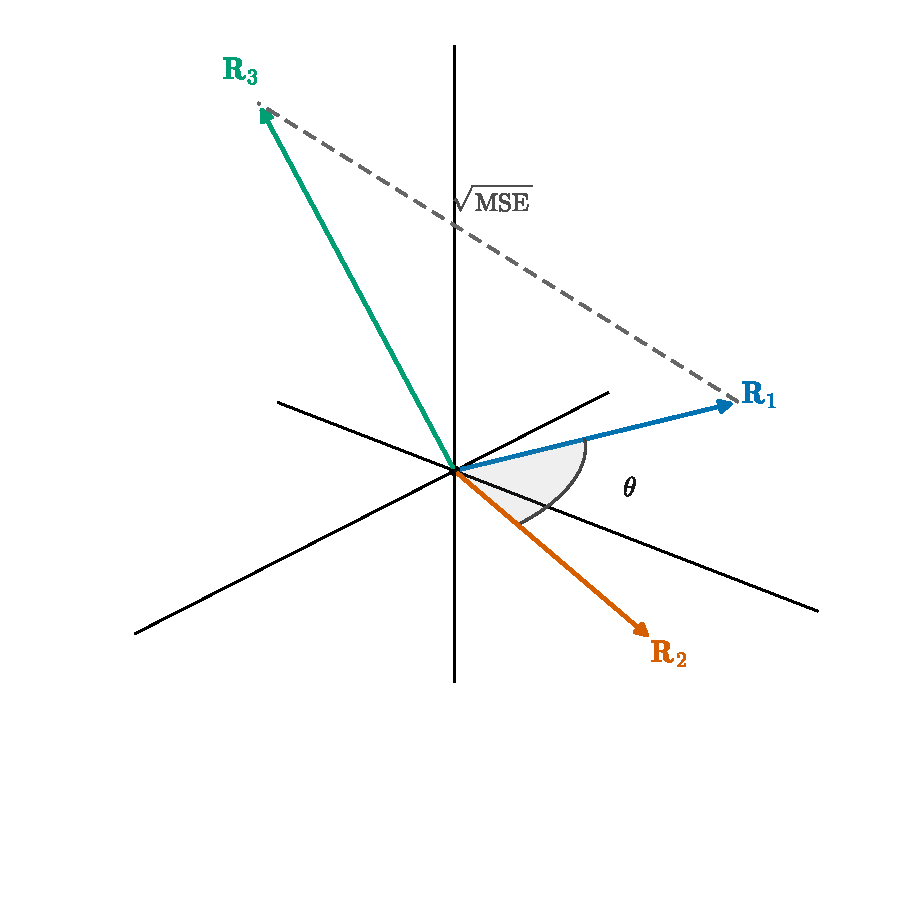
\includegraphics[width=0.5\textwidth]{Figures/hilbert_vectors.pdf}
  \caption{Returns as vectors in $L^2$}
  \label{fig:hilbert}
\end{figure}

Figure \ref{fig:hilbert} is an attempt to represent this abstract space. Now let us
turn to the realized space $\mathbb{R}^T$: the definitions above still apply, bar
the due discretizations, but now we can represent the missing data as a projection
of the full data.
Write:
\[
R_i=P_{\mathcal O_i}R_i+P_{\mathcal M_i}R_i = R_{O_i} + R_{M_i}
\]

Where $P_{\mathcal O_i}$ is the operator that deletes the missing data and $P_{\mathcal M_i}$
is the one that keeps it and deletes the observed one. Their ranges are clearly orthogonal under
the usual inner product.
The goal of our models is to approximate $R_{M_i}$ with:

\[
\hat{R}_{M_i} = h_\theta(R_{O_i}, R_{O_k \neq i})
\]

If we knew the values of $R_{M_i}$ we could run an approximation in the least
squares sense. Given $h_\theta$, find:
\[
\min_\theta\|{R}_{M_i}-\hat{R}_{M_i}\|
\]

This is essentially equivalent to trying to approximate the conditional expectation,
or in geometric terms projecting ${R}_{M_i}$ onto the space of functions $\sigma (R_{O_i}$ and $R_{O_k \neq i})$,
a subspace of $L^2$.

\begin{figure}

  \centering
  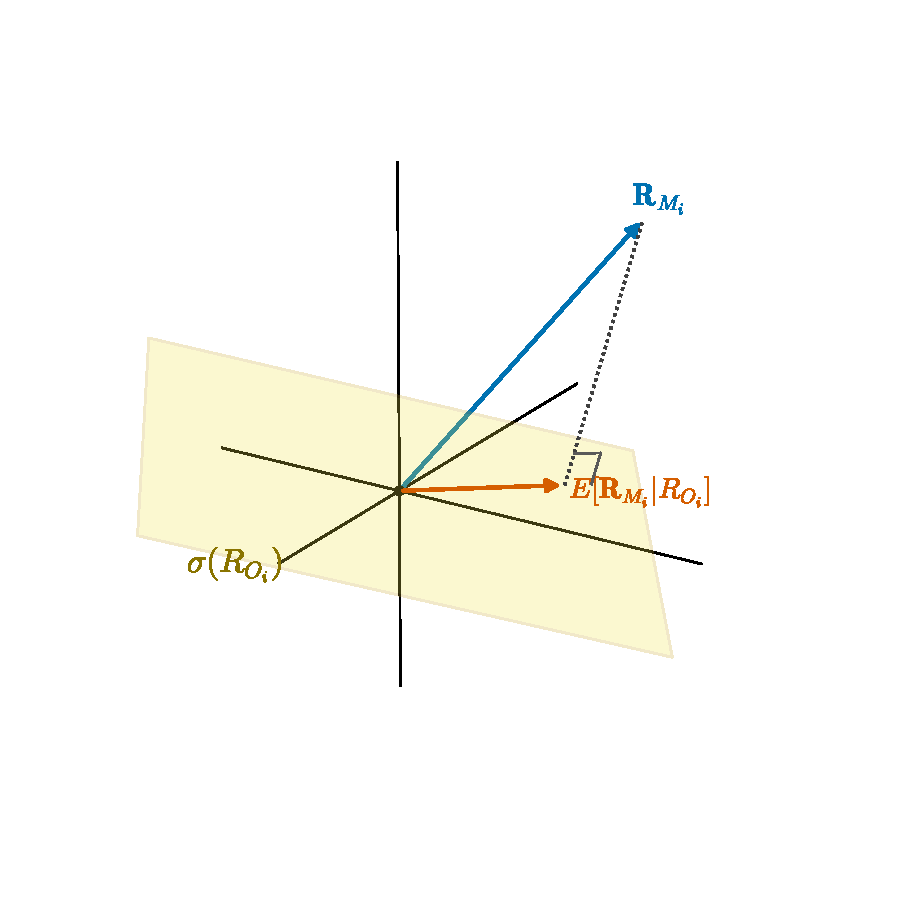
\includegraphics[width=0.7\textwidth]{Figures/projection_H.pdf}
  \caption{Conditional expectation as a projection}
  \label{fig:conditional}
\end{figure}


\clearpage

Let 
\[
R_i=(r_{1i},\ldots,r_{Ti})^\top\in\mathbb R^T
\]
denote the complete return vector of asset \(i\). Suppose that some entries of
\(R_i\) are missing. We denote by
\[
\mathcal O_i=\{t\in\{1,\ldots,T\}: r_{ti}\text{ is observed}\}
\]
the set of observed time indices, and by
\[
\mathcal M_i=\{t\in\{1,\ldots,T\}: r_{ti}\text{ is missing}\}
\]
the set of missing time indices.

For any subset \(A\subseteq\{1,\ldots,T\}\), define the coordinate projection
\(P_A:\mathbb R^T\to\mathbb R^T\) by
\[
(P_A x)_t=
\begin{cases}
x_t, & t\in A,\\
0, & t\notin A.
\end{cases}
\]
Then the complete return vector decomposes as
\[
\boxed{
R_i=P_{\mathcal O_i}R_i+P_{\mathcal M_i}R_i.
}
\]
The first term \(P_{\mathcal O_i}R_i\) is observed, while the second term
\(P_{\mathcal M_i}R_i\) is unobserved.

Under the empirical inner product
\[
\langle X,Y\rangle_T=\frac1T\sum_{t=1}^T X_tY_t,
\]
the two components are orthogonal, because they have disjoint supports:
\[
\left\langle P_{\mathcal O_i}R_i,\,
P_{\mathcal M_i}R_i\right\rangle_T=0.
\]
Hence,
\[
\|R_i\|_T^2
=
\|P_{\mathcal O_i}R_i\|_T^2
+
\|P_{\mathcal M_i}R_i\|_T^2.
\]


\clearpage
A multivariate time series is represented as


Hilbert space

The Hilbert space of square-integrable random variables is



Inner product



Norm

\[
\|X\|
=
\sqrt{\langle X,X\rangle}
=
\sqrt{\mathbb{E}[X^2]}.
\]

Distance

\[
d(X,Y)
=
\|X-Y\|.
\]
Centered random variables

If

\[
\mathbb{E}[X]=0,
\qquad
\mathbb{E}[Y]=0,
\]

then

\[
\langle X,Y\rangle
=
\operatorname{Cov}(X,Y).
\]

Correlation

\[
\rho(X,Y)
=
\frac{\langle X,Y\rangle}
{\|X\|\|Y\|}.
\]

Angle between random variables

\[
\theta
=
\arccos\left(
\frac{\langle X,Y\rangle}
{\|X\|\|Y\|}
\right).
\]
Conditional expectation

Conditional expectation

\[
\mathbb{E}[X\mid\mathcal{G}].
\]

Projection interpretation

\[
\mathbb{E}[X\mid\mathcal{G}]
=
P_{L^2(\mathcal{G})}(X),
\]

where $(P_{L^2(\mathcal{G})})$ denotes the orthogonal projection onto the closed subspace $(L^2(\mathcal{G}))$.

Orthogonality condition

\[
X-
\mathbb{E}[X\mid\mathcal{G}]
\perp
L^2(\mathcal{G}).
\]

Equivalently,

\[
\mathbb{E}
\left[
\left(
X-
\mathbb{E}[X\mid\mathcal{G}]
\right)
Y
\right]
=
0,
\qquad
\forall
Y\in L^2(\mathcal{G}).
\]
Covariance matrix

Mean vector

\[
\mu
=
\mathbb{E}[X].
\]

Covariance matrix

\[
\Sigma
=
\mathbb{E}
\left[
(X-\mu)(X-\mu)^\top
\right].
\]

Sample covariance

\[
S
=
\frac1{T-1}
\sum_{t=1}^T
(x_t-\bar x)
(x_t-\bar x)^\top.
\]

Correlation matrix

\[
R
=
D^{-1/2}
\Sigma
D^{-1/2},
\]

where

\[
D
=
\operatorname{diag}
(\Sigma).
\]
Gram matrix

The Gram matrix of variables

\[
G
=
X^\top X.
\]

The Gram matrix of observations

\[
K
=
XX^\top.
\]
PCA

Eigenvalue decomposition

\[
\Sigma
=
Q
\Lambda
Q^\top.
\]

Projection onto first (k) principal directions

\[
\widehat X
=
XQ_kQ_k^\top.
\]

Low-rank approximation

\[
X
\approx
UV^\top.
\]
Mahalanobis geometry

Mahalanobis distance

\[
d_M(x,\mu)
=
\sqrt{
(x-\mu)^\top
\Sigma^{-1}
(x-\mu)
}.
\]

Squared Mahalanobis distance

\[
\delta
=
(x-\mu)^\top
\Sigma^{-1}
(x-\mu).
\]

Ellipsoid

\[
\mathcal{E}
=
\{
x:
(x-\mu)^\top
\Sigma^{-1}
(x-\mu)
\le c
\}.
\]
Partitioned covariance matrix
\[
\Sigma
=
\begin{pmatrix}
\Sigma_{oo}
&
\Sigma_{om}
\\
\Sigma_{mo}
&
\Sigma_{mm}
\end{pmatrix}.
\]

Conditional mean

\[
\mu_{m|o}
=
\mu_m
+
\Sigma_{mo}
\Sigma_{oo}^{-1}
(x_o-\mu_o).
\]

Conditional covariance

\[
\Sigma_{m|o}
=
\Sigma_{mm}
-
\Sigma_{mo}
\Sigma_{oo}^{-1}
\Sigma_{om}.
\]
Projection matrices

Orthogonal projector

\[
P
=
P^\top
=
P^2.
\]

Least-squares projection

\[
P
=
X
(X^\top X)^{-1}
X^\top.
\]

Projected vector

\[
\widehat y
=
Py.
\]

Residual

\[
r
=
(I-P)y.
\]

Orthogonality

\[
P(I-P)=0.
\]
Matrix norms

Frobenius norm

\[
\|A\|_F
=
\sqrt{
\sum_{i,j}
a_{ij}^2
}.
\]

Spectral norm

\[
\|A\|_2
=
\sigma_{\max}(A).
\]

Nuclear norm

\[
\|A\|_*
=
\sum_i
\sigma_i(A).
\]
Matrix completion

Projection operator

\[
P_\Omega(X).
\]

Optimization problem

\[
\min_M
\;
\frac12
\|
P_\Omega(X-M)
\|_F^2
+
\lambda
\|M\|_*.
\]
Student-(t) distribution
\[
X
\sim
t_\nu(\mu,\Sigma).
\]

Student-(t) weight

\[
w_i
=
\frac{\nu+p}
{\nu+\delta_i}.
\]
EM algorithm

Expected complete-data log-likelihood

\[
Q(\theta|\theta^{(k)})
=
\mathbb{E}
\left[
\log
p(X_{\rm obs},X_{\rm mis}\mid\theta)
\mid
X_{\rm obs},
\theta^{(k)}
\right].
\]

M-step

\[
\theta^{(k+1)}
=
\arg\max_\theta
Q(\theta|\theta^{(k)}).
\]
Random paths

A multivariate path

\[
X:
[0,T]
\rightarrow
\mathbb{R}^N.
\]

Time-parametrized market trajectory

\[
t
\mapsto
X_t.
\]
Signatures

Signature

\[
S(X)
=
\left(
1,
\int dX,
\int dX\otimes dX,
\int dX\otimes dX\otimes dX,
\ldots
\right).
\]

Truncated signature

\[
S^{(m)}(X).
\]

Signature distance

\[
d_{\rm sig}
=
\left\|
S^{(m)}(X)
-
S^{(m)}(\widehat X)
\right\|.
\]
Useful notation

Expectation

\[
\mathbb{E}[X].
\]

Probability

\[
\mathbb{P}(A).
\]

Variance

\[
\operatorname{Var}(X).
\]

Covariance

\[
\operatorname{Cov}(X,Y).
\]

Trace

\[
\operatorname{tr}(A).
\]

Determinant

\[
\det(A).
\]

Rank

\[
\operatorname{rank}(A).
\]

Diagonal matrix

\[
\operatorname{diag}(a_1,\ldots,a_n).
\]

Identity matrix

\[
I_n.
\]

Positive-definite matrices

\[
\mathcal{S}_{++}^n.
\]

Symmetric matrices

\[
\mathcal{S}^n.
\]


\chapter{Results and Discussion}
\label{ch:results}

Tables~\ref{tab:results_sparse}, \ref{tab:results_gaps}
and~\ref{tab:results_stressed} report the seven evaluation metrics of
Section~\ref{sec:eval} for every model, one table per injection pattern of
Section~\ref{sec:missingness}, with the levels ordered by their realised
share of missing cells. Within each level, the best value of every metric is
set in bold. A dash marks a value that is not defined: the pointwise errors
of Deletion (the returned panel changes shape), its remaining metrics at the
heaviest levels (too few complete dates survive), and KNN at the most
extreme stressed level, where the dates to be filled lack well-observed
donors altogether.

Three regularities stand out. First, the hierarchy is stable across
patterns and levels: the conditional methods dominate the two baselines
everywhere, EM is rarely beaten -- and never by much -- while the neural
models match it at a far higher computational cost rather than surpassing
it (BRITS even stumbles at two stressed levels). Second, pointwise and
structural quality diverge exactly as anticipated in
Section~\ref{sec:eval}: under the MCAR patterns mean replacement stays
within roughly fifty per cent of the best MAE while its covariance error is
close to an order of magnitude worse than EM's. Third, MNAR is the
genuinely hostile regime: at the heaviest stressed level no method brings
the relative covariance error below $0.6$ -- the turbulent dates are simply
no longer in the data, and no choice of model recovers them.

\begin{table}[p]
  \centering
  \footnotesize
  \caption{Evaluation scores under sparse missingness (MCAR); levels are the deletion rate $r$.}
  \label{tab:results_sparse}
  \begin{tabular}{llrrrrrrr}
    \toprule
    Level & Model & MAE & RMSE & CovErr & VaRErr & WassErr & AbsACFErr & LevErr \\
    \midrule
    $0.001$ & Deletion & -- & -- & 0.0119 & 0.0001 & 0.0001 & 0.0101 & 0.0114 \\
     & Zero & 0.0118 & 0.0194 & 0.0026 & \textbf{0.0000} & \textbf{0.0000} & 0.0009 & 0.0008 \\
     & KNN & 0.0099 & 0.0168 & 0.0018 & \textbf{0.0000} & \textbf{0.0000} & 0.0006 & 0.0005 \\
     & LowRank & 0.0084 & 0.0152 & 0.0016 & \textbf{0.0000} & \textbf{0.0000} & \textbf{0.0005} & \textbf{0.0004} \\
     & EM & \textbf{0.0080} & \textbf{0.0147} & \textbf{0.0015} & \textbf{0.0000} & \textbf{0.0000} & \textbf{0.0005} & \textbf{0.0004} \\
     & BRITS & 0.0091 & 0.0158 & 0.0016 & \textbf{0.0000} & \textbf{0.0000} & \textbf{0.0005} & \textbf{0.0004} \\
     & CSDI & 0.0081 & 0.0151 & 0.0016 & \textbf{0.0000} & \textbf{0.0000} & \textbf{0.0005} & \textbf{0.0004} \\
    \midrule
    $0.01$ & Deletion & -- & -- & 0.0532 & 0.0005 & 0.0004 & 0.0247 & 0.0334 \\
     & Zero & 0.0107 & 0.0161 & 0.0205 & 0.0001 & 0.0001 & 0.0035 & 0.0027 \\
     & KNN & 0.0081 & 0.0123 & 0.0069 & 0.0001 & \textbf{0.0000} & 0.0019 & 0.0017 \\
     & LowRank & 0.0077 & 0.0117 & 0.0054 & \textbf{0.0000} & \textbf{0.0000} & 0.0016 & 0.0015 \\
     & EM & 0.0071 & 0.0109 & 0.0051 & \textbf{0.0000} & \textbf{0.0000} & \textbf{0.0015} & \textbf{0.0014} \\
     & BRITS & 0.0076 & 0.0116 & 0.0064 & 0.0001 & \textbf{0.0000} & 0.0017 & 0.0016 \\
     & CSDI & \textbf{0.0069} & \textbf{0.0107} & \textbf{0.0050} & \textbf{0.0000} & \textbf{0.0000} & \textbf{0.0015} & \textbf{0.0014} \\
    \midrule
    $0.05$ & Deletion & -- & -- & 0.1951 & 0.0019 & 0.0012 & 0.1334 & 0.0515 \\
     & Zero & 0.0111 & 0.0167 & 0.1044 & 0.0005 & 0.0006 & 0.0132 & 0.0073 \\
     & KNN & 0.0084 & 0.0127 & 0.0283 & 0.0003 & 0.0002 & 0.0047 & 0.0045 \\
     & LowRank & 0.0078 & 0.0118 & 0.0169 & \textbf{0.0002} & \textbf{0.0001} & 0.0045 & 0.0041 \\
     & EM & \textbf{0.0072} & 0.0113 & 0.0151 & \textbf{0.0002} & 0.0002 & 0.0044 & \textbf{0.0039} \\
     & BRITS & 0.0073 & 0.0113 & \textbf{0.0145} & \textbf{0.0002} & 0.0002 & \textbf{0.0043} & 0.0040 \\
     & CSDI & \textbf{0.0072} & \textbf{0.0112} & 0.0149 & \textbf{0.0002} & 0.0002 & 0.0051 & 0.0041 \\
    \midrule
    $0.1$ & Deletion & -- & -- & 0.4492 & 0.0091 & 0.0051 & -- & -- \\
     & Zero & 0.0109 & 0.0163 & 0.1872 & 0.0011 & 0.0011 & 0.0276 & 0.0111 \\
     & KNN & 0.0083 & 0.0125 & 0.0487 & 0.0007 & 0.0004 & 0.0090 & 0.0067 \\
     & LowRank & 0.0077 & 0.0116 & 0.0282 & \textbf{0.0004} & \textbf{0.0003} & 0.0072 & 0.0058 \\
     & EM & \textbf{0.0071} & \textbf{0.0110} & \textbf{0.0237} & 0.0005 & \textbf{0.0003} & \textbf{0.0068} & \textbf{0.0056} \\
     & BRITS & 0.0072 & 0.0111 & 0.0238 & 0.0005 & \textbf{0.0003} & \textbf{0.0068} & 0.0057 \\
     & CSDI & 0.0072 & 0.0111 & 0.0261 & \textbf{0.0004} & \textbf{0.0003} & 0.0077 & 0.0057 \\
    \midrule
    $0.3$ & Deletion & -- & -- & -- & -- & -- & -- & -- \\
     & Zero & 0.0109 & 0.0161 & 0.4749 & 0.0037 & 0.0033 & 0.0638 & 0.0201 \\
     & KNN & 0.0087 & 0.0129 & 0.1467 & 0.0024 & 0.0014 & 0.0173 & 0.0118 \\
     & LowRank & 0.0080 & 0.0119 & 0.0749 & \textbf{0.0014} & \textbf{0.0007} & 0.0170 & 0.0105 \\
     & EM & \textbf{0.0074} & \textbf{0.0112} & 0.0565 & 0.0017 & 0.0009 & 0.0150 & \textbf{0.0099} \\
     & BRITS & 0.0076 & 0.0114 & \textbf{0.0536} & 0.0015 & 0.0008 & \textbf{0.0149} & 0.0101 \\
     & CSDI & \textbf{0.0074} & 0.0113 & 0.0641 & \textbf{0.0014} & 0.0008 & 0.0203 & 0.0112 \\
    \bottomrule
  \end{tabular}
\end{table}

\begin{table}[p]
  \centering
  \footnotesize
  \caption{Evaluation scores under contiguous-gap missingness (MCAR); levels are the parameters $(n, \lambda)$ of Section~\ref{sec:missingness}.}
  \label{tab:results_gaps}
  \begin{tabular}{llrrrrrrr}
    \toprule
    Level & Model & MAE & RMSE & CovErr & VaRErr & WassErr & AbsACFErr & LevErr \\
    \midrule
    $(20,\, 10)$ & Deletion & -- & -- & 0.0103 & 0.0001 & 0.0001 & 0.0033 & 0.0033 \\
     & Zero & 0.0121 & 0.0184 & 0.0027 & \textbf{0.0000} & \textbf{0.0000} & 0.0003 & 0.0002 \\
     & KNN & 0.0096 & 0.0144 & 0.0016 & \textbf{0.0000} & \textbf{0.0000} & 0.0002 & \textbf{0.0001} \\
     & LowRank & 0.0087 & 0.0123 & 0.0010 & \textbf{0.0000} & \textbf{0.0000} & 0.0002 & \textbf{0.0001} \\
     & EM & 0.0079 & 0.0117 & 0.0011 & \textbf{0.0000} & \textbf{0.0000} & \textbf{0.0001} & \textbf{0.0001} \\
     & BRITS & \textbf{0.0078} & \textbf{0.0112} & 0.0010 & \textbf{0.0000} & \textbf{0.0000} & \textbf{0.0001} & \textbf{0.0001} \\
     & CSDI & 0.0079 & 0.0115 & \textbf{0.0009} & \textbf{0.0000} & \textbf{0.0000} & \textbf{0.0001} & \textbf{0.0001} \\
    \midrule
    $(200,\, 10)$ & Deletion & -- & -- & 0.1492 & 0.0010 & 0.0004 & 0.0243 & 0.0158 \\
     & Zero & 0.0107 & 0.0156 & 0.0222 & \textbf{0.0001} & 0.0001 & 0.0037 & 0.0015 \\
     & KNN & 0.0082 & 0.0121 & 0.0065 & \textbf{0.0001} & \textbf{0.0000} & 0.0016 & 0.0012 \\
     & LowRank & 0.0078 & 0.0118 & 0.0061 & \textbf{0.0001} & \textbf{0.0000} & 0.0015 & 0.0012 \\
     & EM & \textbf{0.0072} & \textbf{0.0109} & \textbf{0.0046} & \textbf{0.0001} & \textbf{0.0000} & \textbf{0.0014} & \textbf{0.0011} \\
     & BRITS & 0.0073 & 0.0111 & 0.0049 & \textbf{0.0001} & \textbf{0.0000} & 0.0015 & \textbf{0.0011} \\
     & CSDI & \textbf{0.0072} & \textbf{0.0109} & 0.0049 & \textbf{0.0001} & \textbf{0.0000} & 0.0015 & \textbf{0.0011} \\
    \midrule
    $(1000,\, 10)$ & Deletion & -- & -- & 0.1825 & 0.0017 & 0.0010 & 0.1135 & 0.0493 \\
     & Zero & 0.0104 & 0.0152 & 0.0785 & 0.0004 & 0.0005 & 0.0155 & 0.0048 \\
     & KNN & 0.0080 & 0.0118 & 0.0224 & 0.0003 & 0.0002 & 0.0059 & 0.0032 \\
     & LowRank & 0.0074 & 0.0108 & 0.0137 & \textbf{0.0002} & \textbf{0.0001} & \textbf{0.0048} & 0.0029 \\
     & EM & \textbf{0.0069} & \textbf{0.0103} & 0.0116 & \textbf{0.0002} & \textbf{0.0001} & 0.0049 & 0.0028 \\
     & BRITS & 0.0070 & 0.0104 & 0.0116 & \textbf{0.0002} & \textbf{0.0001} & 0.0049 & 0.0028 \\
     & CSDI & \textbf{0.0069} & \textbf{0.0103} & \textbf{0.0114} & \textbf{0.0002} & \textbf{0.0001} & 0.0051 & \textbf{0.0027} \\
    \midrule
    $(1000,\, 20)$ & Deletion & -- & -- & 0.8524 & 0.0087 & 0.0042 & 0.1872 & 0.1681 \\
     & Zero & 0.0110 & 0.0163 & 0.1716 & 0.0010 & 0.0010 & 0.0354 & 0.0068 \\
     & KNN & 0.0085 & 0.0127 & 0.0487 & 0.0007 & 0.0004 & 0.0117 & 0.0049 \\
     & LowRank & 0.0078 & 0.0119 & 0.0310 & \textbf{0.0004} & \textbf{0.0003} & 0.0088 & 0.0046 \\
     & EM & \textbf{0.0073} & \textbf{0.0114} & \textbf{0.0238} & 0.0005 & \textbf{0.0003} & 0.0083 & \textbf{0.0044} \\
     & BRITS & 0.0074 & \textbf{0.0114} & 0.0241 & 0.0005 & \textbf{0.0003} & \textbf{0.0082} & 0.0045 \\
     & CSDI & \textbf{0.0073} & 0.0115 & 0.0328 & \textbf{0.0004} & \textbf{0.0003} & 0.0095 & \textbf{0.0044} \\
    \midrule
    $(2000,\, 30)$ & Deletion & -- & -- & 1.4799 & 0.0104 & 0.0100 & -- & -- \\
     & Zero & 0.0108 & 0.0161 & 0.4324 & 0.0028 & 0.0027 & 0.0908 & 0.0143 \\
     & KNN & 0.0085 & 0.0128 & 0.1378 & 0.0018 & 0.0011 & 0.0277 & 0.0090 \\
     & LowRank & 0.0080 & 0.0120 & 0.0820 & \textbf{0.0010} & \textbf{0.0006} & 0.0218 & 0.0083 \\
     & EM & \textbf{0.0073} & \textbf{0.0113} & 0.0589 & 0.0012 & 0.0007 & 0.0212 & \textbf{0.0079} \\
     & BRITS & 0.0074 & 0.0114 & \textbf{0.0555} & 0.0011 & \textbf{0.0006} & \textbf{0.0187} & 0.0082 \\
     & CSDI & 0.0074 & 0.0115 & 0.0896 & \textbf{0.0010} & 0.0007 & 0.0265 & 0.0091 \\
    \bottomrule
  \end{tabular}
\end{table}

\begin{table}[p]
  \centering
  \footnotesize
  \caption{Evaluation scores under stressed missingness (MNAR); levels are the parameters $(r, h, p)$ of Section~\ref{sec:missingness}.}
  \label{tab:results_stressed}
  \begin{tabular}{llrrrrrrr}
    \toprule
    Level & Model & MAE & RMSE & CovErr & VaRErr & WassErr & AbsACFErr & LevErr \\
    \midrule
    $(0,\, 0.1,\, 0.99)$ & Deletion & -- & -- & 0.2813 & 0.0009 & 0.0004 & 0.0582 & 0.0200 \\
     & Zero & 0.0552 & 0.0640 & 0.0676 & 0.0001 & 0.0001 & 0.0115 & 0.0070 \\
     & KNN & 0.0202 & 0.0285 & 0.0229 & \textbf{0.0000} & \textbf{0.0000} & 0.0034 & 0.0029 \\
     & LowRank & 0.0158 & 0.0220 & 0.0116 & \textbf{0.0000} & \textbf{0.0000} & 0.0025 & 0.0020 \\
     & EM & \textbf{0.0133} & \textbf{0.0187} & \textbf{0.0094} & \textbf{0.0000} & \textbf{0.0000} & \textbf{0.0021} & \textbf{0.0017} \\
     & BRITS & 0.0301 & 0.0385 & 0.0253 & \textbf{0.0000} & \textbf{0.0000} & 0.0046 & 0.0036 \\
     & CSDI & 0.0163 & 0.0226 & 0.0175 & \textbf{0.0000} & \textbf{0.0000} & 0.0027 & 0.0022 \\
    \midrule
    $(0.005,\, 0.5,\, 0.99)$ & Deletion & -- & -- & 0.2960 & 0.0010 & 0.0005 & 0.0687 & 0.0268 \\
     & Zero & 0.0321 & 0.0463 & 0.2238 & 0.0005 & 0.0003 & 0.0483 & 0.0172 \\
     & KNN & 0.0161 & 0.0261 & 0.0991 & 0.0001 & \textbf{0.0001} & 0.0168 & 0.0095 \\
     & LowRank & 0.0129 & 0.0200 & \textbf{0.0279} & \textbf{0.0000} & \textbf{0.0001} & 0.0078 & 0.0067 \\
     & EM & \textbf{0.0118} & \textbf{0.0189} & 0.0319 & \textbf{0.0000} & \textbf{0.0001} & \textbf{0.0077} & \textbf{0.0065} \\
     & BRITS & 0.0122 & 0.0197 & 0.0401 & \textbf{0.0000} & \textbf{0.0001} & 0.0082 & 0.0069 \\
     & CSDI & 0.0136 & 0.0233 & 0.0751 & \textbf{0.0000} & \textbf{0.0001} & 0.0132 & 0.0087 \\
    \midrule
    $(0.04,\, 0.2,\, 0.95)$ & Deletion & -- & -- & 0.5325 & 0.0043 & 0.0018 & 0.1079 & 0.0491 \\
     & Zero & 0.0143 & 0.0219 & 0.2254 & 0.0010 & 0.0007 & 0.0375 & 0.0143 \\
     & KNN & 0.0092 & 0.0141 & 0.0562 & 0.0003 & 0.0002 & 0.0092 & 0.0067 \\
     & LowRank & 0.0083 & 0.0125 & 0.0253 & \textbf{0.0002} & \textbf{0.0001} & 0.0068 & 0.0052 \\
     & EM & \textbf{0.0077} & \textbf{0.0117} & \textbf{0.0217} & \textbf{0.0002} & \textbf{0.0001} & \textbf{0.0062} & \textbf{0.0048} \\
     & BRITS & 0.0078 & 0.0118 & 0.0231 & \textbf{0.0002} & \textbf{0.0001} & 0.0064 & 0.0049 \\
     & CSDI & 0.0078 & 0.0122 & 0.0374 & \textbf{0.0002} & \textbf{0.0001} & 0.0078 & 0.0061 \\
    \midrule
    $(0.05,\, 0.5,\, 0.9)$ & Deletion & -- & -- & 0.6318 & 0.0056 & 0.0023 & 0.1230 & 0.0630 \\
     & Zero & 0.0174 & 0.0249 & 0.5125 & 0.0030 & 0.0017 & 0.0843 & 0.0244 \\
     & KNN & 0.0103 & 0.0161 & 0.1602 & 0.0010 & 0.0004 & 0.0258 & 0.0124 \\
     & LowRank & 0.0091 & 0.0139 & \textbf{0.0483} & \textbf{0.0004} & \textbf{0.0002} & 0.0110 & 0.0091 \\
     & EM & \textbf{0.0084} & \textbf{0.0130} & 0.0554 & 0.0008 & 0.0003 & \textbf{0.0107} & \textbf{0.0087} \\
     & BRITS & 0.0106 & 0.0162 & 0.2083 & 0.0015 & 0.0006 & 0.0256 & 0.0126 \\
     & CSDI & 0.0086 & 0.0137 & 0.0542 & 0.0008 & 0.0003 & 0.0165 & 0.0109 \\
    \midrule
    $(0.2,\, 1,\, 0.9)$ & Deletion & -- & -- & -- & -- & -- & -- & -- \\
     & Zero & 0.0149 & 0.0219 & 0.7677 & 0.0070 & 0.0042 & 0.1201 & 0.0333 \\
     & KNN & -- & -- & -- & -- & -- & -- & -- \\
     & LowRank & 0.0137 & 0.0212 & 0.6525 & \textbf{0.0062} & 0.0029 & 0.1111 & 0.0316 \\
     & EM & \textbf{0.0134} & \textbf{0.0210} & 0.6634 & 0.0065 & 0.0031 & 0.1112 & 0.0315 \\
     & BRITS & 0.0136 & 0.0214 & \textbf{0.6480} & 0.0063 & \textbf{0.0025} & 0.1069 & 0.0299 \\
     & CSDI & \textbf{0.0134} & \textbf{0.0210} & 0.6559 & 0.0064 & 0.0028 & \textbf{0.1065} & \textbf{0.0298} \\
    \bottomrule
  \end{tabular}
\end{table}

\section{Computational costs}




\chapter{Conclusion}
\label{ch:conclusion}

\section{Summary}

\section{Limitations}

\section{Future Work}

\cleardoublepage
\addcontentsline{toc}{chapter}{Bibliography}
\bibliography{references}

\listoffigures
\addcontentsline{toc}{chapter}{List of Figures}
\cleardoublepage

\listoftables
\addcontentsline{toc}{chapter}{List of Tables}
\cleardoublepage

\end{document}
